%%%%%%%%%%%%%%%%%%%%%%%%%%%%%%%%%%%%%%%%%%%%%%%%%%%%%%%%%%%%%%%%%%%%%%%%
\chapter{Background}
\label{chapter:background}
%%%%%%%%%%%%%%%%%%%%%%%%%%%%%%%%%%%%%%%%%%%%%%%%%%%%%%%%%%%%%%%%%%%%%%%%
\localtableofcontents
\vspace{\marginbellowtable}

This chapter gives a short introduction on the theory of supervised learning~\cite{shalev2014understanding} and Toeplitz matrices~\cite{gray2006toeplitz}.
In the statistical learning framework, supervised learning refers to the notion of learning the parameters of a specific function that maps an input to an output based on example input-output pairs.
For example, an image (input) associated with its content: label (output).
The first section describe a formal model that aims to describe such learning tasks.
In linear algebra, a Toeplitz matrix, named after Otto Toeplitz, is a matrix in which each descending diagonal from left to right is constant.
The second section describe the mathematical properties of Toeplitz matrices and known theorems that we use in this thesis. 


%%%%%%%%%%%%%%%%%%%%%%%%%%%%%%%%%%%%%%%%%%%%%%%%%%%%%%%%%%%%%%%%%%%%%%%%%%%%%%%
\section{Introduction on Supervised Learning}
\label{section:ch2-introduction_on_supervised_learning}
%%%%%%%%%%%%%%%%%%%%%%%%%%%%%%%%%%%%%%%%%%%%%%%%%%%%%%%%%%%%%%%%%%%%%%%%%%%%%%%

\begin{figure}[h]
  \centering
  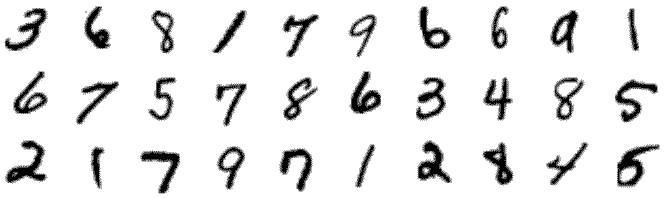
\includegraphics[width=0.85\textwidth]{figures/main/ch2-background/mnist-dataset.png}
  \caption{Images with handwritten digits in the MNIST database \cite{lecun1998gradient}}
  \label{figure:ch2-mnist-database}
\end{figure}


In \citeyear{lecun1998gradient}, \citeauthor{lecun1998gradient} had successfully learn a function capable of recognizing handwritten digits in images.
They used the MNIST database \cite{lecun1998gradient} which consists of black and white images of size $28 \times 28$ pixels (see Figure~\ref{figure:ch2-mnist-database}).
Their goal was to build a machine that take a vector as input and produce the identity of the digit $0 \dots 9$ as the output.
This is a nontrivial problem because each image is unique and while digits can be differentiated based on their shapes and strokes, these features gives poor results for an automated system. 

In the following, we will formalize the learning problem describe above with the \emph{statistical learning framework}.
First, let us define the domain space $\mathcal{X} = [0, 1]^n$ of of dimension $n$.
The domain space corresponds to the set of images that we wish to label.
In our example above, this domain corresponds to the whole to the set of all handwritten number images.
Let us denote the label space $\mathcal{Y} = [k]$ where $k$ is the number of class and a finite sequence of pairs $\mathcal{S} = \left\{ \left(\xvec^{(1)}, y^{(1)} \right) \dots \left( \xvec^{(m)}, y^{(m)} \right) \right\}$ in $\mathcal{X} \times \mathcal{Y}$. 
Such pairs \ie, labeled examples, are called \emph{training examples} and the set $\mathcal{S}$ is called the \emph{training set}.
We denote $\mathcal{D}$ the \emph{joint distribution} over $\mathcal{X} \times \mathcal{Y}$.
The main objective of the task at hand is to output a \emph{prediction rule} $h: \mathcal{X} \rightarrow \mathcal{Y}$ that maps the input $\xvec \in \mathcal{X}$ to the output $y \in \mathcal{Y}$.
This function is called the \emph{hypothesis} or the \emph{classifier}. 
Given the probability distribution $\mathcal{D}$, we aim to measure how \emph{likely} the hypothesis $h$ make an error when labeled points are randomly drawn from the distribution $\mathcal{D}$.
Let us define the true error of \emph{risk} of the hypothesis $h$
\begin{equation}
  R_{\mathcal{D}}(h) \triangleq \Pbb_{(\xvec, y) \sim \mathcal{D}} \left[ h(\xvec) \neq  y \right] 
  \label{equation:ch2-risk1}
\end{equation}
However, in practice, the joint probability distribution $\mathcal{D}$ is unknown, therefore, the true error is not directly available to the learner.
The learner only has access to the training data, $\mathcal{S}$, and can calculate the \emph{empirical error} \ie, the error over the training samples.
We define the \emph{empirical risk} as follows:
\begin{equation}
  R_{\mathcal{S}}(h) \triangleq \frac{\left| \left\{i \in [m]: h\left(\xvec^{(i)}\right) \neq y^{(i)} \right\}\right|}{m}
\end{equation}
We can generalize our measure of correctness so that it can be applied to multiple learning tasks.
Let us define a \emph{loss function} from $\mathcal{H} \times \mathcal{D}$ to the set of nonnegative real numbers, $L: \mathcal{H} \times \mathcal{D} \rightarrow \Rbb^{+}$.
We can define the \emph{risk} as follows:
\begin{equation}
  R_{\mathcal{D}}(h) \triangleq \Ebb_{(\xvec, y) \sim \mathcal{D}} \left[ L(h(\xvec), y) \right] \enspace.
  \label{equation:ch2-risk2}
\end{equation}
Similarly, we define the empirical risk as follows:
\begin{equation}
  R_{\mathcal{S}}(h) \triangleq \frac{1}{m} \sum_{(\xvec, y) \sim \mathcal{S}} L(h(\xvec), y) \enspace.
\end{equation}
The loss functions used for classification problems and regression problems are as follows: 
\begin{itemize}
  \item \textbf{0-1 Loss}: $L_{0-1}(h, (\xvec, y)) = \mathds{1}\left[ h(\xvec) = y \right]$ \\
  This loss is used for classification problems, for example, when the learner have to recognizing hand-written digits in images.
  We can notice that the definitions of $R_{\mathcal{D}}$ given in Equation~\ref{equation:ch2-risk1} and Equation~\ref{equation:ch2-risk2} coincide with our loss for classification problems.
  \item \textbf{Square Loss}: $L_{\text{sq}}(h, (\xvec, y)) = \left((h(\xvec) - y \right)^2$ \\	
  This loss is used for another common type of learning problem \ie, \emph{regression problem}, in which the label domain $\mathcal{Y}$ is the set of real numbers.
  For example, one wishes to predict the price of an apartment given its characteristics.
\end{itemize}


\noindent
The goal of the learning algorithm is to find the hypothesis $h$ that minimize the risk $R_{\mathcal{S}}$, this learning paradigm is called \emph{Empirical Risk Minimization} (ERM).
We use the ERM paradigm as a surrogate to find an hypothesis $h$ that minimize the true risk $R_\mathcal{D}$.
However, all hypothesis that minimize the empirical error does not necessarily minimize the true risk.
For example, consider the following function:
\begin{equation}
  h^* =
  \begin{cases}
    1 \quad \text{if }\exists i \in [n] \text{ s.t. } \xvec_i  = \xvec \\
    0 \quad \text{otherwise}
  \end{cases}
  \label{equation:ch2-perfect_function}
\end{equation}
Clearly, this function, for any sample $\mathcal{S}$, will have $R_\mathcal{S}(h^*) = 0$, whereas the true risk will certainly be high.
The phenomenon of \emph{overfitting} happens when the classifier fits the training data ``too well'' but will likely have a high error on unseen data.
One possible solution to this phenomenon is to apply ERM with a restricted search space to prevent the learning algorithm to output a function such as $h^*$ in Equation~\ref{equation:ch2-perfect_function}.
We call this set the \emph{hypothesis class} and is denoted $\mathcal{H}$. 
Each $h \in \mathcal{H}$ is a function mapping from $\mathcal{X}$ to $\mathcal{Y}$.
We call $\mathrm{ERM}_{\mathcal{H}}$, the learned that use the $\mathrm{ERM}$ paradigm over the hypothesis class $\mathcal{H}$ and a training data $\mathcal{S}$.
Formally,
\begin{equation}
  \mathrm{ERM}_{\mathcal{H}}(\mathcal{S}) \in \argmin_{h \in \mathcal{H}} R_{\mathcal{S}}(h) \enspace.
\end{equation}
For a training sample $\mathcal{S}$, we denote $h_\mathcal{S}$, one solution of applying $\text{ERM}_\mathcal{H}$ on the set $\mathcal{S}$, if there exists multiple hypotheses with minimal error on the training sample, then minimization problem returns an arbitrary one.
In practice, the hypothesis class is chosen based on an hypothesis on the relation between the data and its label.
For example, if the relation between the data and its label is supposedly linear then the hypothesis class can be the set of all linear function.
This kind of restriction is called an \emph{inductive bias} because we the learner is \emph{biased} towards a particular set of predictors.

\begin{figure}[h]
  \centering
  \begin{subfigure}[b]{0.32\textwidth}
    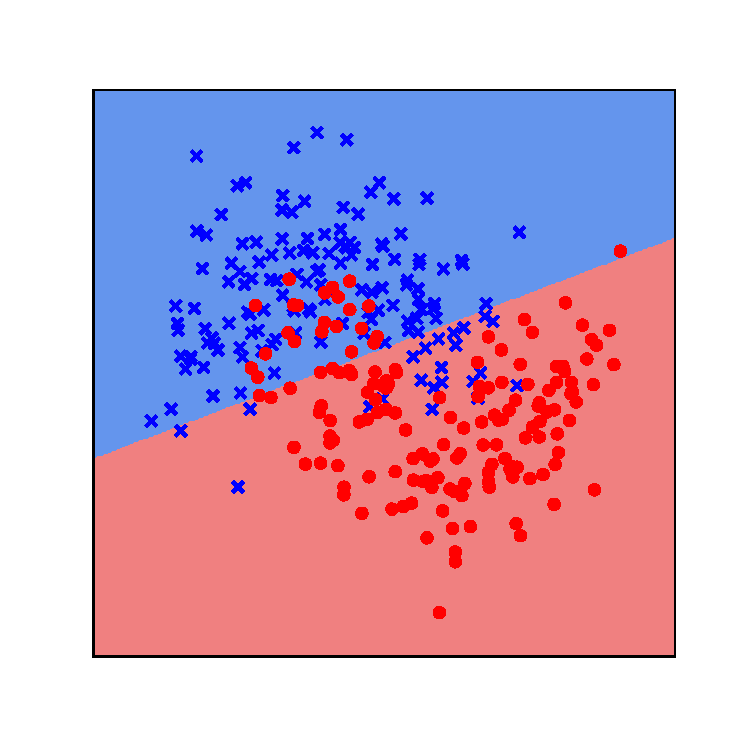
\includegraphics[width=0.98\textwidth]{figures/main/ch2-background/underfitting.pdf}
    \caption{Underfitting}
    \label{figure:ch2-fitting_points_a}
  \end{subfigure}
  \hfill
  \begin{subfigure}[b]{0.32\textwidth}
    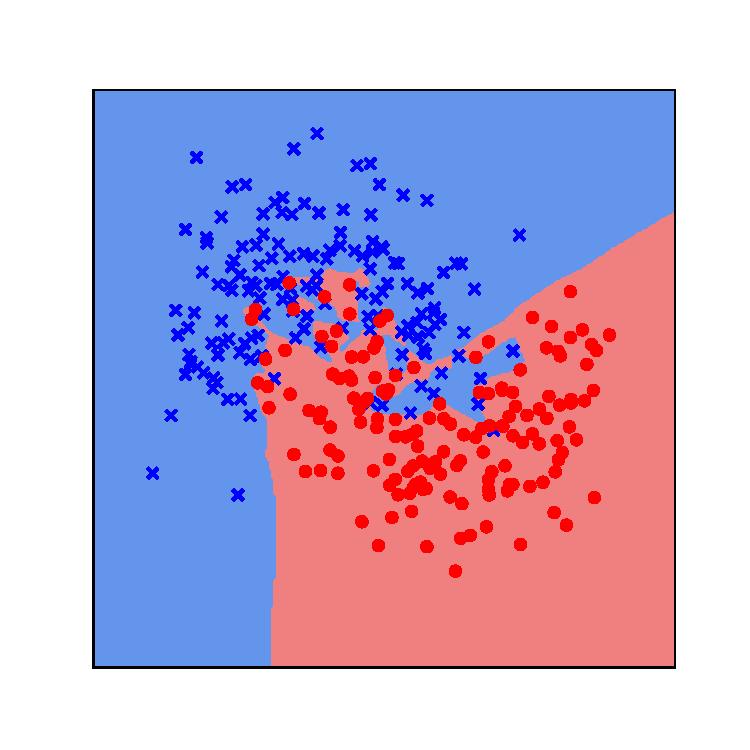
\includegraphics[width=0.98\textwidth]{figures/main/ch2-background/overfitting.pdf}
    \caption{Overfitting}
    \label{figure:ch2-fitting_points_b}
  \end{subfigure}
  \hfill
  \begin{subfigure}[b]{0.32\textwidth}
    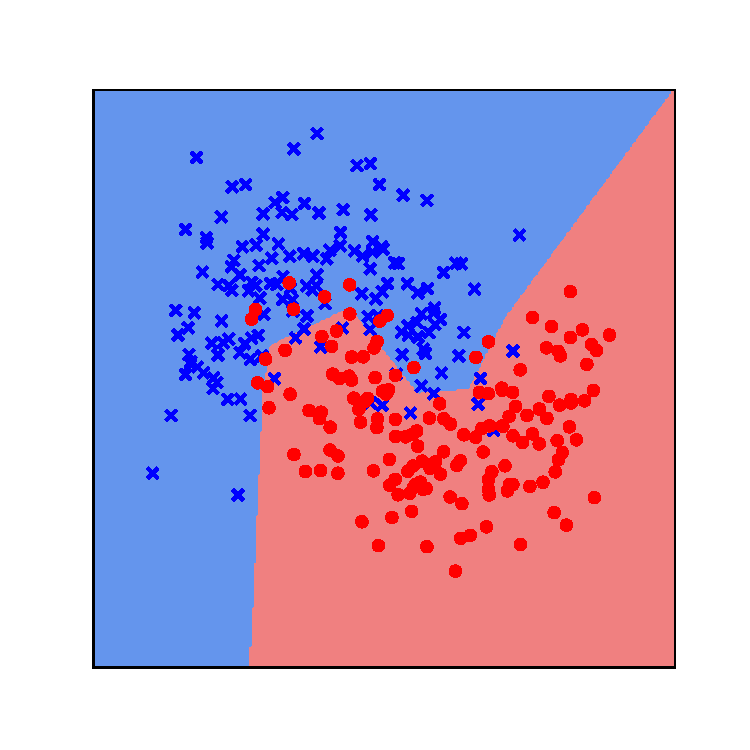
\includegraphics[width=0.98\textwidth]{figures/main/ch2-background/normal.pdf}
    \caption{Good fit}
    \label{figure:ch2-fitting_points_c}
  \end{subfigure}
  \caption{
    Decision boundary of 3 classifiers with different complexity for the same set of sample.
  }
  \label{figure:ch2-fitting_points}
\end{figure}


A fundamental question remain is, \emph{how to choose the correct hypothesis class for which $\text{ERM}_\mathcal{H}$ will not lead to overfitting?} 
We answer this question by decomposing the true risk into two different components as follows: 
\begin{equation}
  R_\mathcal{D} (h_\mathcal{S}) = 
  \underbrace{\left[ \min_{h \in \mathcal{H}} R_\mathcal{D}(h) \right]}_{\text{\scriptsize Approximation Error}} + \quad 
  \underbrace{\left[ R_\mathcal{D}(h_\mathcal{S}) - \min_{h \in \mathcal{H}} R_\mathcal{D}(h) \right]}_{\text{\scriptsize Estimation Error}} 
  \label{equation:ch2-bias_complexity_tradeoff}
\end{equation}
\begin{itemize}
  \item \textbf{Approximation Error}: The approximation error corresponds to the minimum risk achievable by a classifier in the given hypothesis class.
  Intuitively, this error measure the quality of the hypothesis class and therefore the quality of the prior knowledge.
  Enlarging the hypothesis class, \ie, allowing more complex functions, can decrease the approximation error.
  \item \textbf{Estimation Error}: The estimation error is the difference between the approximation error and the error made by the ERM predictor.
  Recall that the empirical risk is only an estimate of the true risk
  This error is dependent of the sample size and/or the complexity of the hypothesis class. 
\end{itemize}
Recall that the main goal is to minimize the true risk $R_\mathcal{D} (h_\mathcal{S})$, however, Equation~\ref{equation:ch2-bias_complexity_tradeoff} shows a tradeoff called the \emph{bias-complexity tradeoff}. 
The tradeoff is as follows: if we choose a large and complex hypothesis space, we reduce the approximation error but at the same time can increase the estimation error because a complex hypothesis space might lead to overfitting.
Conversely, choosing a small hypothesis space might reduce the reduce the estimation error but increase the approximation error leading to an \emph{underfitting} phenomenon.
We can demonstrate the \emph{overfitting} and \emph{underfitting} phenomenons with Figure~\ref{figure:ch2-fitting_points} which shows the decision boundary of 3 classifiers for the same set of samples.
Figure~\ref{figure:ch2-fitting_points_a} shows a classifier which \emph{underfit} the data, meaning the decision boundary is not complex enough to separate the data correctly. 
The Figure~\ref{figure:ch2-fitting_points_b} shows a classifier that almost perfectly follows the training data but is likely to have a higher error rate on the unseen data
Finally, the Figure~\ref{figure:ch2-fitting_points_c} shows a classifier that seems to have a good compromise between the two.

As seen above, defining a small hypothesis class might lead to underfitting and a large hypothesis class might lead to overfitting.
A good way to offset a large hypothesis class would be to specific preference over hypothesis within the hypothesis class.
The \emph{Structural Minimization Paradigm} (SRM) assume that the hypothesis class can be written as the union of multitude smaller hypothesis class as follows: $\mathcal{H} = \bigcup_{n \in \Nbb} \mathcal{H}_n$ with a weight function $w: \Nbb \rightarrow [0, 1]$ which assigns a weight to each hypothesis class, $\mathcal{H}_n$, such that a higher weights reflects a lower preference for the hypothesis class.
The SRM learning paradigm can then be updated as follows:
\begin{equation}
  \text{SRM}_\mathcal{H} \in \argmin_{h \in \mathcal{H}, n \in \Nbb} \left[ R_\mathcal{S}(h) + w(n) \right]
\end{equation}
This learning algorithm will minimize the empirical risk $R_\mathcal{S}(h)$ and by minimizing the weight function $w$ will output an hypothesis that belong to a preferred hypothesis class. 
In the next section, we will see the type of hypothesis we want to learn and how to implement the ERM and SRM paradigm.




\drawline






\drawline




The ERM paradigm with inductive bias is based on an important assumption.
We assume that uniformly over all $h \in \mathcal{H}$, the empirical risk is close to the true risk, meaning, an $h$ that minimize the empirical risk with respect to a data set $\mathcal{S}$ will also minimize the \emph{true} risk.
More formally, 
\begin{equation}
  \forall h \in \mathcal{H}, \quad \left| R_\mathcal{S}(h) - R_\mathcal{D}(h) \right| \leq \epsilon \enspace.
  \label{equation:ch2-eps_respresentative_sample} 
\end{equation}
If this assumption is met, then the ERM paradigm will always return a good classifier. 
\begin{lemma}[Lemma 4.2 \citet{shalev2014understanding}] 
  If Equation~\ref{equation:ch2-eps_respresentative_sample} hold, then any output of $\mathrm{ERM}_\mathcal{H}(\mathcal{S})$, namely, any $h_\mathcal{S} \in \argmin_{h \in \mathcal{H}} R_\mathcal{S}(h)$, satisfies
  \begin{equation}
    R_\mathcal{D}(h_\mathcal{S}) \leq \min_{h \in \mathcal{H}} R_\mathcal{S}(h) + 2\epsilon
  \end{equation}
\end{lemma}









% However, any classifier $h$ that minimize $R_{\mathcal{S}}$

% The ERM paradigm has an important drawback.

% however, this function would obtain a high error on

% The ERM paradigm has been known to led to \emph{overfitting} \ie, the empirical error is i

% the classifier performs perfectly on the training data, yet performs poorly on ``true'' data.





\todo{SRM and regularization}



% Let us consider an input space $\mathcal{X} = [0, 1]^d$ of dimension $d$, an output space $\mathcal{Y} = [k]$ where $k$ is the number of class and a data distribution $\mathcal{D}$ over $\mathcal{X} \times \mathcal{Y}$.
% We seek to find a function $h: \mathcal{X} \rightarrow \mathcal{Y}$ that maps the input $\xvec \in \mathcal{X}$ to the output $y \in \mathcal{Y}$ with $h \in \mathcal{H}$ where $h$ is called the \emph{hypothesis} and $\mathcal{H}$ the \emph{hypothesis space}.
% in order to measure how well the function fits, we de\emph{loss function} $l: \mathcal{y} \times \mathcal{y} \rightarrow \rbb^{+}$ is defined.
% The \emph{risk} $R$ associated with the hypothesis $h(\xvec)$ is defined as follows:
% \begin{equation}
%   R(h) \triangleq \Ebb_{(\xvec, y) \sim \mathcal{D}}\  L \left( h(\xvec), y \right)
% \end{equation}
% The goal of a \emph{learning algorithm} is to find an hypothesis $h^* \in \mathcal{H}$ which minimize the risk $R(h)$:
% \begin{equation}
%   h^* \triangleq \argmin_{h \in \mathcal{H}} R(h) .
% \end{equation}

% In practice, the joint probability distribution $\mathcal{D}$ is unknown.
% Instead, we have $n$ independent observations of the distribution called the \emph{training set}
% \begin{equation}
%   \mathcal{T} \triangleq \left\{ \left(\xvec^{(1)}, y^{(1)} \right), \dots, \left( \xvec^{(n)}, y^{(n)} \right) \right\} ,
% \end{equation}
% where $\xvec \in \mathcal{X}$ and $y \in \mathcal{Y}$.

% The risk minimization problem is therefore replace by the \emph{empirical risk minimization} as follows:
% \begin{equation}
%   E(h, n) \triangleq \frac{1}{n} \sum_{i = 1}^{n} L\left(h\left(\xvec^{(i)}\right), y^{(i)}\right) ,
% \end{equation}
% the learning algorithm then becomes:
% \begin{equation}
%   \hat{h}^* \triangleq \argmin_{h \in \mathcal{H}} E(h, n)  .
% \end{equation}


% \paragraph{Structural Risk Minimization} (SRM).
% The ERM principle assumes that the function $\hat{h}^*$ minimizing $E(h, n)$ leads to the risk $R(\hat{h}^*)$ being close to the minimum.
% This assumption mean that as the \emph{size} of the training set increase the minimization becomes more accurate. More formally, the ERM principle assumes that $R(\hat{h}^*)$ converge to its minimum value on the set $h \in \mathcal{H}$ when $n \rightarrow \infty$.  
% \citet{Vapnik1991TheNA} have shown that this equivalent to say that the empirical risk $E(h, n)$ \emph{converge uniformly} to the actual risk $R(h)$ over $h \in \mathcal{H}$ where the \emph{uniform convergence} is defined as follows:
% \begin{equation}
%   \Pbb \left[ \sup_{h \in \mathcal{H}} \left| R(h) - E(h, n) \right| < \epsilon \right] \rightarrow 0 \quad \text{ when } \quad n \rightarrow \infty, \quad \forall \epsilon > 0 
% \end{equation}


% \citet{Vapnik1991TheNA} have shown that this assumption is equivalent to the following: does the empirical risk $E(h, n)$ \emph{converge uniformly} to the actual risk $R(h)$ over $h \in \mathcal{H}$ where the \emph{uniform convergence} is defined as follows:
% \begin{equation}
%   \Pbb \left[ \sup_{h \in \mathcal{H}} \left| R(h) - E(h, n) \right| < \epsilon \right] \rightarrow 0 \quad \text{ when } \quad n \rightarrow \infty, \quad \forall \epsilon > 0 
% \end{equation}


% However, does increasing the \emph{size} of the training set allow a better minimisation of the actual risk. More formally, does $R(\hat{h}^*)$ converge to its minimum value on the set $h \in \mathcal{H}$ when $n \rightarrow \infty$. 

% \citet{vapnik1992principles} 

% The 0-1 loss function is a natural loss function to use because it assigns 0 for a correct classification and 1 for an incorrect classification. 


% of the ERM principle \ie, does $R(\hat{h}^*)$ converge to its minimum value on the set $h \in \mathcal{H}$ when $n \rightarrow \infty$ is equivalent to the question: 

% is equivalent to the question: does the empirical risk E(h, n) \emph{converge uniformly} to the actual risk $R(h)$ over $h \in \mat

% \begin{equation}
%   h^* = \argmin_{h \in \mathcal{H}} \frac{1}{n} \sum_{i = 0}^{n} L(h(\xvec_i), y) + \lambda C(\theta) 
% \end{equation}

% Because the relation between $\xvec \in \mathcal{X}$ and $y \in \mathcal{Y}$ is unknown, we aim to find the best approximation of the function $h$ with a parameterized function $h_\theta \in \mathcal{H}$ where $\mathcal{H}$ is called the \emph{hypothesis space}.

% The goal of a \textbf{learning algorithm} is to learn a function $f: \mathcal{X} \rightarrow \mathcal{Y}$ which outputs $y \in \mathcal{Y}$ given an input $\xvec \in \mathcal{X}$ with $f \in \mathcal{H}$ where $\mathcal{H}$ is called the \emph{hypothesis space}.

% The supervised learning settings assume that a function $f: \mathcal{X} \rightarrow \mathcal{Y}$ exists. 

% The supervised learning settings assume that a function $f$ that maps $\xvec \sim \mathcal{X}$ to $y \sim \mathcal{y}$ exists. 

% The goal of a \textbf{learning algorithm} is to approximate $f$ by a parameterized function $f_\theta$.
% The standard method to learn the set of parameters $\theta$ is the \textbf{empirical risk minimization (ERM)}:
% \begin{equation*}
%   \hat{\theta}_{ERM} \triangleq \argmin_{\theta} \frac{1}{n} \sum_{i=1}^{n} L (f_{\theta} (\xvec_i), y_i )
% \end{equation*}

% \begin{equation}
%   \min_{\theta} \Ebb_{(\xvec, y) \sim \mathcal{D}} \left[ L(f_\theta(x), y) \right]. 
% \end{equation}

\newpage

%%%%%%%%%%%%%%%%%%%%%%%%%%%%%%%%%%%%%%%%%%%%%%%%%%%%%%%%%%%%%%%%%%%%%%%%%%%%%%%
\section{Neural Networks}
\label{subsection:ch2-neural_networks}
%%%%%%%%%%%%%%%%%%%%%%%%%%%%%%%%%%%%%%%%%%%%%%%%%%%%%%%%%%%%%%%%%%%%%%%%%%%%%%%

% \item description of neural networks
% \item ERM rule of neural network are NP-Hard
% \item SGD and Backpropagation

% Feedfoward neural network 
% Convolutional neural network


% In practice, the hypothesis class is chosen based on an hypothesis on the relation between the data and its label.
% For example, if the relation between the data and its label is supposedly linear then the hypothesis class can be the set of all linear function.
% This kind of restriction is called an \emph{inductive bias} because we the learner is \emph{biased} towards a particular set of predictors.



In the previous section, we said that we restrict the learner towards a specific set of predictors.
In this thesis, we will focus on neural networks. 
Neural networks, which find their roots in the work of \citet{mcculloch1943logical,rosenblatt1958perceptron}, can be analytically described as a composition of linear functions interlaced with non-linear functions (also called activation functions).
A neural network can be defined as follows:

\begin{definition}[Neural Network]
  A neural network is a function $f^{\rho}_{\Wmat, \Bmat} : \Rbb^{n} \rightarrow \Rbb^{k}$ such that
  \begin{equation}
    f^{\rho}_{\Wmat,\Bmat}(\xvec) \triangleq \phi^{\rho}_{\Wmat^{(d)}, \bvec^{(d)}} \circ \cdots \circ \phi^{\rho}_{\Wmat^{(1)}, \bvec^{(1)}}(\xvec)
  \end{equation}
  where $d$ corresponds to the depth of the network (\ie, the number of layers), $\Wmat$ is the set of weights matrices $\Wmat = \left\{ \Wmat^{(1)} \dots \Wmat^{(d)} \right\}$, $\Bmat$ is the set of bias vectors $\Bmat = \left\{ \bvec^{(1)} \dots \bvec^{(d)} \right\}$. 
  $\phi^{\rho}_{\Wmat^{(i)},\bvec^{(i)}}$ (also called layer) is a function parameterized by the weight matrix $\Wmat^{(i)}$, the bias vector $\bvec^{(i)}$ and the activation function $\rho$ and can be expressed as follows: 
  \begin{equation}
    \phi^{\rho}_{\Wmat^{(i)},\bvec^{(i)}} (\xvec) \triangleq \rho\left(\Wmat^{(i)}\xvec + \bvec^{(i)}\right)
  \end{equation}
\end{definition}



\todo{SRM with hypothesis neural network and SGD}



% \noindent
% Based on this definition, the set of all neural networks is parameterized by the set of weights matrices $\Wmat$, the set of all bias vector $\Bmat$ and an activation function $\rho$.


% The input space $n$ corresponds to the dimension of the data and the output space $m$ corresponds to the number of classes the network has to classify.



\begin{figure}[t]
  \centering
  \begin{subfigure}[b]{0.32\textwidth}
    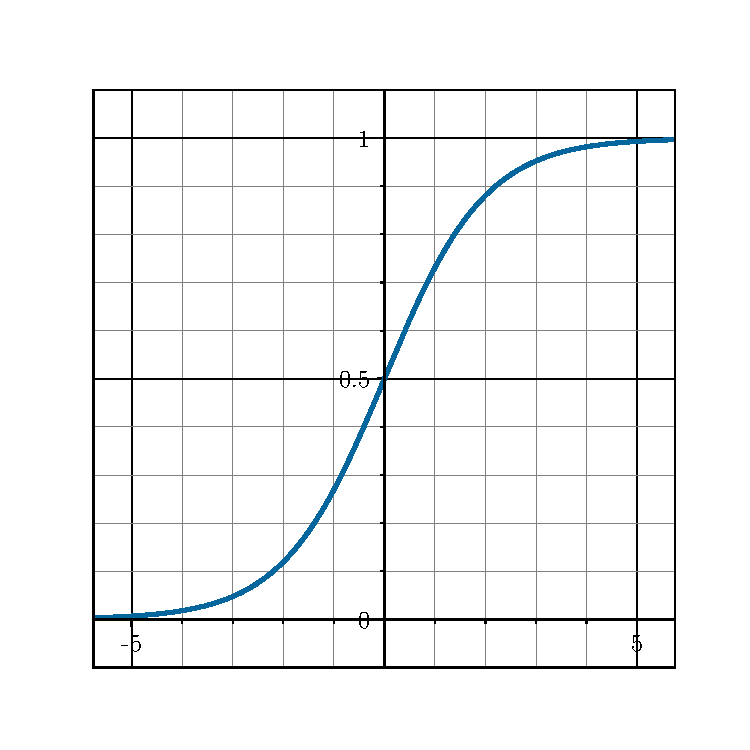
\includegraphics[width=0.98\textwidth]{figures/main/ch2-background/sigmoid.pdf}
    \caption{Sigmoid Activation}
  \end{subfigure}
  \hfill
  \begin{subfigure}[b]{0.32\textwidth}
    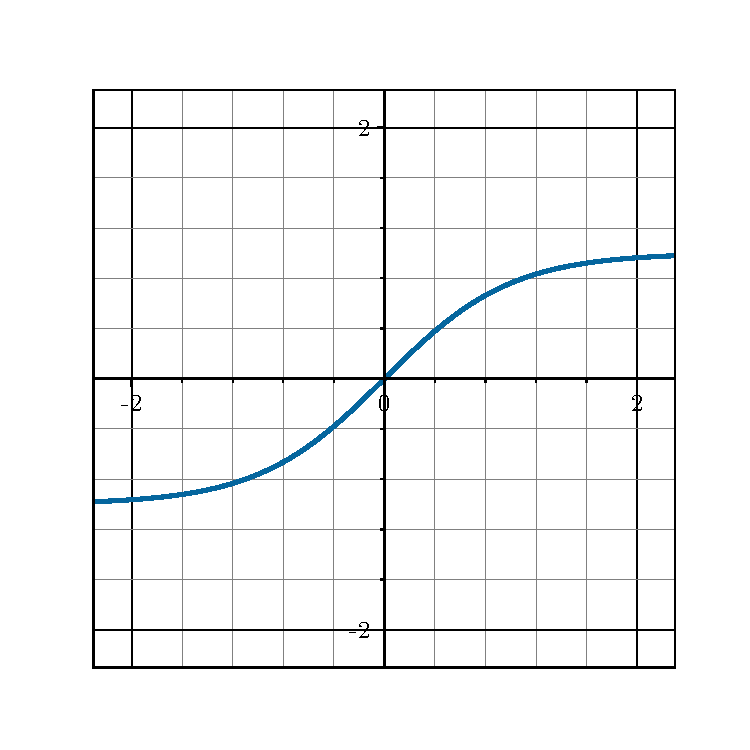
\includegraphics[width=0.98\textwidth]{figures/main/ch2-background/tanh.pdf}
    \caption{Tanh Activation}
  \end{subfigure}
  \hfill
  \begin{subfigure}[b]{0.32\textwidth}
    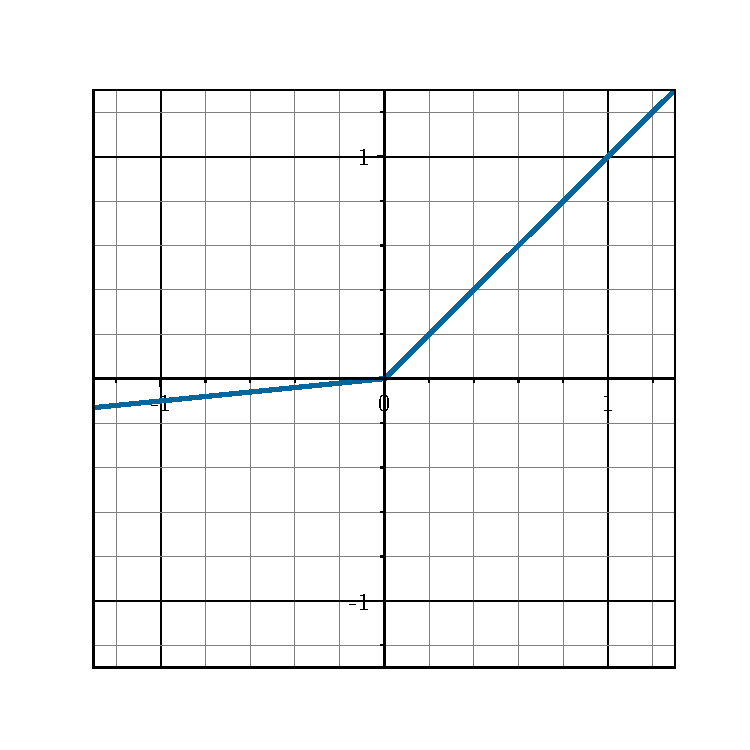
\includegraphics[width=0.98\textwidth]{figures/main/ch2-background/relu.pdf}
    \caption{Leaky ReLU Activation}
  \end{subfigure}
  \caption{Graphical representation of 3 common activation functions}
  \label{figure:ch2-activation_functions}
\end{figure}

\noindent
Choosing the right activation function has been an active area of research. 
Hereafter, we present 3 common activation functions used by practitioners.
\begin{itemize}
  \item \textbf{Sigmoid activation} \cite{han1995influence}
    \begin{equation*}
      \rho(x) = \frac{1}{1+e^{-x}} 
    \end{equation*}
    The sigmoid activation function is one of the first continuous non-linear function to be used in the context of neural network. It takes a real value as input and outputs another value between 0 and 1.
  \item \textbf{Hyperbolic Tangent activation} \cite{karlik2011performance}
    \begin{equation*}
      \rho(x) = \frac{e^x - e^{-x}}{e^x + e^{-x}}
    \end{equation*}
    The hyperbolic tangent activation function is similar to the sigmoid activation function but instead of returning between 0 and 1, the function returns between -1 and 1.     
  \item \textbf{Leaky Rectified Linear activation (Leaky-ReLU)} \cite{maas2013rectifier}
    \begin{equation*}
      \rho(x) = \max(\alpha, x)
    \end{equation*}
    More recently, the ReLU~\cite{nair2010rectified} ($\alpha = 0$) and leaky-ReLU~\cite{maas2013rectifier} ($\alpha > 0$) activation function was proposed.
    The parameter $\alpha$ characterize the slope on $\Rbb_-$.
    These function have the advantages to avoids the vanishing gradient problem and are less less computationally expensive than tanh and sigmoid because it involves simpler mathematical operations.
\end{itemize}

\noindent
The Figure~\ref{figure:ch2-activation_functions} present the graphical representation of the 3 activation functions presented above.
In this thesis, we will exclusively use the Leaky-ReLU function with different $\alpha$ when we train deep neural networks.
Therefore, we simplify the notation $f^{\rho}_{\Wmat, \Bmat}$ with $f_{\Wmat, \Bmat}$.




\drawline


%   where $\phi_{\Wmat^{(i)},\bvec^{(i)}} \triangleq \rho\left(\Wmat^{(i)}\xvec + \bvec^{(i)}\right)$ and $\rho$ is the non-linear function.
%
% \begin{equation}
%   f_{\Theta,\Bmat}(\xvec) \triangleq \phi_{\Wmat^{(L)}, \bvec^{(L)}} \circ \cdots \circ \phi_{\Wmat^{(1)}, \bvec^{(1)}}(\xvec)
% \end{equation}


% \drawline 
% $\rightarrow$ ERM rule of neural network are NP-Hard
%
% $\rightarrow$ SGD and Backpropagation


% During the training of the neural network, the backpropagation algorithm \emph{efficiently} computes the gradient of the loss function we seek to minimize allowing the training of multi layer neural network. In practice, the backpropagation algorithm is simply an application of the chain rule for the composition of function. If $h$, $f$ and $g$ are differentiable functions and $h(x) = (f \circ g)(x)$ then:
% \begin{equation}
%   h'(x) = (f \circ g)' = (f' \circ g) \cdot g'.
% \end{equation}

\newpage

%%%%%%%%%%%%%%%%%%%%%%%%%%%%%%%%%%%%%%%%%%%%%%%%%%%%%%%%%%%%%%%%%%%%%%%%%%%%%%%
\section{Preliminaries on Adversarial Attacks}
\label{section:ch2-preliminaries_on_adversarial_attacks}
%%%%%%%%%%%%%%%%%%%%%%%%%%%%%%%%%%%%%%%%%%%%%%%%%%%%%%%%%%%%%%%%%%%%%%%%%%%%%%%

Deep neural networks achieve state-of-the-art performances in a variety of domains such as natural language processing~\cite{radford2018Language}, image recognition~\cite{he2016deep} and speech recognition~\cite{hinton2012deep}.
However, it has been shown that such neural networks are vulnerable to \emph{adversarial examples}, \ie, imperceptible variations of the natural examples, crafted to deliberately mislead the models~\cite{globerson2006nightmare,biggio2013evasion,szegedy2013intriguing}.
Since their discovery, a variety of algorithms have been developed to generate adversarial examples (\aka attacks), for example FGSM \cite{goodfellow2014explaining}, PGD \cite{madry2018towards} and C\&W \cite{carlini2017towards}, to mention the most popular ones.

Because it is difficult to characterize the space of visually imperceptible variations of a natural image, existing adversarial attacks use surrogates that can differ from one attack to another.
For example, \citet{goodfellow2014explaining} use the $\linf$ norm to measure the distance between the original image and the adversarial image whereas \citet{carlini2017towards} use the $\ltwo$ norm.
When the input dimension is low, the choice of the norm is of little importance because the $\linf$ and $\ltwo$ balls overlap by a large margin, and the adversarial examples lie in the same space.
An important insight in this paper is to observe that the overlap between the two balls  diminishes exponentially quickly as the dimensionality of the input space increases.
For typical image datasets with large dimensionality, the two balls are mostly disjoint.
As a consequence, the $\linf$ and the $\ltwo$ adversarial examples lie in different areas of the space, and it explains why $\linf$ defense mechanisms perform poorly against $\ltwo$ attacks and vice versa. 

\%\%

An \textbf{Adversarial Attack} aims to find the worst perturbation $\tau$ with $\norm{\tau}_p \leq \epsilon$ in such a way that the Neural Network misclassifies. Therefore, an attacker aims to find the solution to the following problem:
\begin{equation}
  \tau_{\theta}^{\mathrm{adv}}(\xvec) \triangleq \max_{\norm{\tau}_p \leq \epsilon} \mathcal{L}(\mathcal{N}_\theta(\xvec + \tau), y)
\end{equation}

\%\%




%%%%%%%%%%%%%%%%%%%%%%%%%%%%%%%%%%%%%%%%%%%%%%%%%%%%%%%%%%%%%%%%%%%%%%%%%%%%%%%
\subsection{Implementing Adversarial Attacks}
\label{subsection:ch2-adversarial_attacks}
%%%%%%%%%%%%%%%%%%%%%%%%%%%%%%%%%%%%%%%%%%%%%%%%%%%%%%%%%%%%%%%%%%%%%%%%%%%%%%%
 
Given an input-output pair $(\xvec, y) \sim \mathcal{D}$, an \emph{adversarial attack} is a procedure that produces a small perturbation $\pmb{\tau} \in  \mathcal X$  such that $f_\theta(\xvec + \pmb{\tau}) \neq y$.
To find the best perturbation $\pmb{\tau}$, existing attacks can adopt one of the two following strategies:
\begin{itemize}
  \item \textbf{Loss maximization}: maximizing the loss $L(f_\theta(\xvec + \pmb{\tau}), y)$ under some constraint on $\norm{\pmb{\tau}}_p$ with $p \in \{0, \cdots, \infty\}$.;
  \item \textbf{Perturbation minimization}: minimizing $\norm{\pmb{\tau}}_p$ under some constraint on the loss $L(f_\theta(\xvec + \pmb{\tau}), y)$.
\end{itemize}

\paragraph{Loss maximization.}
In this scenario, the procedure maximizes the loss objective function, under the constraint that the $\lp$ norm of the perturbation remains bounded by some value $\epsilon$, as follows:  
\begin{equation}
  \argmax_{\norm{\pmb{\tau}}_p \leq \epsilon} L(f_\theta(\xvec + \pmb{\tau}), y) \enspace.
  \label{equation:ch2-lossmax}
\end{equation}
The typical value of $\epsilon$ depends on the norm $\norm{\cdot}_p$ considered in the problem setting.
In order to compare $\linf$ and $\ltwo$ attacks of similar strength, we choose values of $\epsilon_\infty$ and $\epsilon_2$ (for $\linf$ and $\ltwo$ norms respectively) which result in $\linf$ and $\ltwo$ balls of equivalent volumes.
For the particular case of CIFAR-10, this would lead us to choose $\epsilon_\infty = 0.03$ and $\epsilon_2 = 0.8$ which correspond to the maximum values chosen empirically to avoid the generation of visually detectable perturbations. 
The current state-of-the-art method to solve Problem~(\ref{equation:ch2-lossmax}) is based on a projected gradient descent (PGD)~\cite{madry2018towards} of radius~$\epsilon$. Given a budget $\epsilon$, it recursively computes
\begin{equation}
  \xvec^{t+1}=\prod_{B_p(\xvec,\epsilon)}\left(\xvec^t
  +\alpha \argmax_{\delta \text{ s.t. } \norm{\delta}_p \leq 1} \left( \Delta^t \ |\ \delta \right)\right)
  \label{equation:ch2-projectionPGD}
\end{equation}
where $B_p(\xvec,\epsilon) = \{ \xvec + \pmb{\tau} \text{ s.t. } \norm{\pmb{\tau}}_p \leq \epsilon\}$, $\Delta^t = \nabla_\xvec L\left( f_\theta \left(\xvec^t \right), y \right)$, $\alpha$ is a gradient step size, and $\prod_S$ is the projection operator on $S$. Both PGD attacks with $p=2$, and $p=\infty$ are currently used in the literature as state-of-the-art attacks for the loss maximization problem. 

\paragraph{Perturbation minimization.}
This type of procedure search for the perturbation that has the minimal $\lp$ norm, under the constraint that $L(f_\theta(\xvec + \pmb{\tau}), y)$ is bigger than a given bound $c$:
\begin{equation}
  \argmin_{L(f_\theta(\xvec + \pmb{\tau}), y) \geq c} \norm{\pmb{\tau}}_p \enspace.
  \label{equation:ch2-normmin}
\end{equation}
The value of $c$ is typically chosen depending on the loss function $L$. For example, if $L$ is the $0/1$ loss, any $c > 0$ is acceptable.
Problem~\ref{equation:ch2-normmin} has been tackled by~\citet{carlini2017towards}, leading to the following method, denoted C\&W attack in the rest of the chapter. It aims at solving the following Lagrangian relaxation of Problem~\ref{equation:ch2-normmin}:
\begin{equation}
  \argmin_{\pmb{\tau}} \norm{\pmb{\tau}}_p+ \lambda \times g(\xvec+\pmb{\tau})
\end{equation}
where $g(x+\pmb{\tau})<0$ if and only if $L(f_\theta(x+\pmb{\tau}),y) \geq c$. 
The authors use a change of variable $\pmb{\tau}=\tanh(w)-x$ to ensure that $-1 \leq x+\pmb{\tau} \leq 1$, a binary search to optimize the constant $c$, and Adam or SGD to compute an approximated solution.
The C\&W attack is well defined both for $p=2$, and $p=\infty$, but there is a clear empirical gap of efficiency in favor of the $\ltwo$ attack.


%%%%%%%%%%%%%%%%%%%%%%%%%%%%%%%%%%%%%%%%%%%%%%%%%%%%%%%%%%%%%%%%%%%%%%%%%%%%%%%
\subsection{Defending against Adversarial Attacks}
\label{subsection:ch2-defending_against_adversarial_attacks}
%%%%%%%%%%%%%%%%%%%%%%%%%%%%%%%%%%%%%%%%%%%%%%%%%%%%%%%%%%%%%%%%%%%%%%%%%%%%%%%

Adversarial Training was introduced by~\citet{goodfellow2014explaining} and later improved by~\citet{madry2018towards} as a first defense mechanism to train robust neural networks.
It consists in augmenting training batches with adversarial examples generated during the training procedure.
The risk minimization principled is thus replaced by the following $\min$ $\max$ problem, where the classifier tries to minimize the expected loss under maximum perturbation of its input:
\begin{equation}
  \min_{\theta} \Ebb_{(\xvec, y) \sim \mathcal{D}} \left[ \max_{\norm{\pmb{\tau}}_p \leq \epsilon} L \left( f_{\theta}(\xvec + \pmb{\tau}), y \right) \right].
\end{equation}


\%\%\%

\cite{goodfellow2014explaining} have proposed \textbf{Adversarial Training} which follows \textbf{ERM} training over adversarially-perturbed samples
\begin{equation}
  \argmin_{\theta} \frac{1}{n} \sum_{i=1}^{n} \mathcal{L} (\mathcal{N}_\theta (\xvec_i + \tau_{\theta}^{\mathrm{adv}}(\xvec_i)), y_i)
\end{equation}


\%\%\%

In the case where $p = \infty$, this technique offers good robustness against $\linf$ attacks \cite{athalye2018obfuscated}.
The main weakness of Adversarial Training is its lack of formal guarantees.
Despite some recent work providing great insights \cite{sinha2017certifying,zhang2019theoretically}, there is no worst case lower bound yet on the accuracy under attack of this method.

\todo{make a small reference to noise injection technique and cite appendix}

% Another important technique to defend against adversarial examples is to use Noise Injection. 
% In contrast with Adversarial Training, Noise Injection mechanisms are usually deployed after training.
% In a nutshell, it works as follows.
% At inference time, given a unlabeled sample $x$, the network outputs
% \begin{equation}
%   \tilde{f}_\theta(\xvec) \triangleq f_\theta(\xvec + \eta) \ \ \ (\text{instead of  } f_\theta(\xvec)) 
% \end{equation}
% where $\eta$ is a random variable on $\mathbb{R}^d$.
% Even though, Noise Injection is often less efficient than Adversarial Training in practice (see \eg, Table~\ref{table:764774}), it benefits from strong theoretical background.
% In particular, recent works \cite{lecuyer2018certified,li2019certified}, followed by~\citet{cohen2019certified,pinot2019theoretical} demonstrated that noise injection from a Gaussian distribution can give provable defense against $\ltwo$ adversarial attacks.
% In this work, besides the classical Gaussian noises already investigated in previous works, we evaluate the efficiency of Uniform distributions to defend against $\ltwo$ adversarial examples. 



\newpage

%%%%%%%%%%%%%%%%%%%%%%%%%%%%%%%%%%%%%%%%%%%%%%%%%%%%%%%%%%%%%%%%%%%%%%%%%%%%%%%
\section{A Primer on Toeplitz and Circulant Matrices}
\label{section:ch2-a_primer_on_toeplitz_and_circulant_matrices}
%%%%%%%%%%%%%%%%%%%%%%%%%%%%%%%%%%%%%%%%%%%%%%%%%%%%%%%%%%%%%%%%%%%%%%%%%%%%%%%

% $=>$ introduction on Toeplitz matrices and their generating function
% $=>$ Circulant Matrix is a special case of Toeplitz matrices 
% $=>$ Presenting block circulant and block Toeplitz
% $=>$ After introduction circulant matrices, present theorem for bound the singular values of Toeplitz and Toeplitz matrices 

%%%%%%%%%%%%%%%%%%%%%%%%%%%%%%%%%%%%%%%%%%%%%%%%%%%%%%%%%%%%%%%%%%%%%%%%%%%%%%%
\subsection{Toeplitz Matrices}
\label{subsection:ch2-toeplitz_matrices}
%%%%%%%%%%%%%%%%%%%%%%%%%%%%%%%%%%%%%%%%%%%%%%%%%%%%%%%%%%%%%%%%%%%%%%%%%%%%%%%

A Toeplitz matrix, named after Otto Toeplitz, is a matrix in which each descending diagonal from left to right is constant.
An $n\times n$ Toeplitz matrix $\Amat$ is fully determined by a two-sided sequence of scalars $\{a_\seqidx\}_{\seqidx \in \seqsetN}$ as follows:

\begin{equation}
  \Amat =
  \leftmatrix
    a_0 & a_{1} & a_{2} & \cdots & \cdots & a_{n-1} \\
    a_{-1} & a_0 & a_{1} & \ddots & & \vdots \\
    a_{-2} & a_{-1} & \ddots & \ddots & \ddots & \vdots \\ 
    \vdots & \ddots & \ddots & \ddots & a_{1} & a_{2} \\
    \vdots & & \ddots & a_{-1} & a_{0} & a_{1} \\
    a_{-n+1} & \cdots & \cdots & a_{-2} & a_{-1} & a_0
  \rightmatrix
\end{equation}

\noindent
Because the Toeplitz matrix $\Amat$ is fully determined by the sequence $\{\Amat_h\}_{h \in N}$, it can be compactly represented in memory using only $2n-1$ values instead of $n^2$.
Toeplitz matrices can also be characterized by noting that the $(k,j)$ entry of $\Amat$, $\Amat_{j,k}$ is given by
\begin{equation}
  \Amat_{j,k} = a_{k-j} \enspace.
\end{equation}

\noindent
A standard tool for manipulating Toeplitz matrices is the use of Fourier analysis.
Let $\{a_\seqidx\}_{\seqidx \in \seqsetN}$ be the sequence of coefficients of the Toeplitz matrix $\Amat \in \mathbb{R}^{n\times n}$.
The complex-valued function 
\begin{equation}
  f(\omega) = \sum_{\seqidx \in \seqsetN} a_\seqidx e^{\ci \seqidx \omega}
\end{equation}
is the \emph{inverse Fourier transforms} of the sequences $\{a_\seqidx\}_{\seqidx \in \seqsetN}$ with $\omega \in \mathbb{R}$.
From this function, one can recover the sequence $\{a_\seqidx\}_{\seqidx \in \seqsetN}$ using the standard Fourier transform:
\begin{equation}
  a_\seqidx = \frac{1}{2\pi} \int_0^{2\pi} e^{-\ci \seqidx \omega} f(\omega) d\omega \enspace. 
\end{equation}

\noindent
From there, similarly to the work done by~\citet{gray2006toeplitz}, we can define an operator $\Tmat$ mapping integrable functions to matrices:
\begin{equation}
  \Tmat(g) \triangleq \leftmat\frac{1}{2\pi}\int_{0}^{2\pi}e^{-\ci(i-j)\omega}g(\omega)\,d\omega\rightmat_{i,j\in\{0,\ldots,n-1\}} \enspace.
  \label{equation:ch2-toeplitz_operator}
\end{equation}

\noindent
We can show that if $f$ is the inverse Fourier transform of $\{a_\seqidx\}_{\seqidx \in \seqsetN}$, then $\Tmat(f)$ is equal to $\Amat$.
\begingroup
\allowdisplaybreaks
  \begin{align}
      \leftmat \Tmat(f) \rightmat_{i, j} &= \frac{1}{2\pi} \int_0^{2\pi} e^{-\ci (i-j)\omega} f(\omega) \,d\omega  \\
      &= \frac{1}{2\pi} \int_0^{2\pi} e^{-\ci (i-j) \omega} \sum_{h \in N} a_h e^{\ci h \omega} \,d\omega  \\
      &= \frac{1}{2\pi} \int_0^{2\pi} \sum_{h \in N} a_h e^{\ci (j - i + h) \omega} \,d\omega  \\
      &= \sum_{h \in N} a_h \frac{1}{2\pi} \int_0^{2\pi} e^{\ci (j - i + h) \omega} \,d\omega 
      = a_{j-i} .
  \end{align}
\endgroup
Because:
\begin{equation}
  \frac{1}{2\pi} \int_0^{2\pi} e^{\ci k \omega} \,d\omega = 
  \begin{cases}
    1 \quad \text{if}\ k = 0, \\
    0 \quad \text{if}\ k\ \text{is a non-zero integer number.}
  \end{cases}
\end{equation}

% Also, if $F$ is the inverse Fourier transform of $\{\Bmat_\seqidx\}_{\seqidx \in \seqsetN}$ as defined above, then the integral in Equation~\ref{equation:expression_toeplitz_matrix} is matrix-valued, and thus $\Tmat(F) \in \mathbb{R}^{mn \times mn}$ is the block matrix $\Bmat$.

% The trigonometric polynomial that \emph{generates} the Toeplitz matrix $\Amat$ can be defined as follows:
% \begin{equation}
%   f_{\Amat}(\omega) \triangleq \sum_{h \in N} a_h e^{\ci h \omega}
% \end{equation}
% The function $f_{\Amat}$ is said to be the \emph{generating function} of $\Amat$.
% To recover the Toeplitz matrix from its generating function, we have the following operator:
% \begin{equation}
%   \leftmat \Tmat(f) \rightmat_{i, j} \triangleq \frac{1}{2\pi} \int_0^{2\pi} e^{-\ci (i - j)\omega} f(\omega) \,d\omega .
%   \label{equation:ch2-toeplitz_operator}
% \end{equation}


%%%%%%%%%%%%%%%%%%%%%%%%%%%%%%%%%%%%%%%%%%%%%%%%%%%%%%%%%%%%%%%%%%%%%%%%%%%%%%%
\subsection{Circulant Matrices}
\label{subsection:ch2-circulant_matrices}
%%%%%%%%%%%%%%%%%%%%%%%%%%%%%%%%%%%%%%%%%%%%%%%%%%%%%%%%%%%%%%%%%%%%%%%%%%%%%%%

Circulant matrices are a special case of Toeplitz matrices.
In addition to having constant diagonals, each row of a circulant matrix is a cyclic right shift of the previous one.
% Circulant matrices have been used to efficiently solve linear systems~\cite{golub1996matrix} and years later were used to perform dimensionality reduction~\cite{hinrichs2011johnson,vybiral2011variant}, binary embedding~\cite{yu2014circulant} and kernel approximation~\cite{yu2015compact} in the context of pattern recognition and machine learning.
An $n \times n$ circulant matrix $\Cmat$ is fully determined by a sequence of scalars $\{c_h\}_{h \in [n]}$ as follows:

\begin{equation}
  \Cmat =
  \leftmatrix
    c_0 & c_{n-1} & c_{n-2} & \cdots & \cdots & c_{1} \\
    c_{1} & c_0 & c_{n-1} & \ddots & & \vdots \\
    c_{2} & c_{1} & \ddots & \ddots & \ddots & \vdots \\ 
    \vdots & \ddots & \ddots & \ddots & c_{n-1} & c_{n-2} \\
    \vdots & & \ddots & c_{1} & c_{0} & c_{n-1} \\
    c_{n-1} & \cdots & \cdots & c_{2} & c_{1} & c_0
  \rightmatrix
\end{equation}

\noindent
because the circulant matrix $\Cmat$ is fully determined by the sequence $\{c_h\}_{h \in [n]}$, it can be compactly represented in memory using only $n$ values instead of $n^2$.
Circulant matrices can also be characterized by noting that the $(k,j)$ entry of $\Cmat$, $\Cmat_{j,k}$ is given by
\begin{equation}
  \Cmat_{j,k} = c_{\left(k-j\right) \mod n} \enspace.
\end{equation}
Circulant matrices exhibit several interesting properties which are based on the fact that they can be diagonalized by the Discrete Fourier Transform (DFT)~\cite{davis1979circulant}.
More precisely, the eigenvalues $\psi_k$ of the matrix $\Cmat$ correspond to the discrete Fourier transform of the vector characteristic $\cvec$:
\begin{equation}
  \mathbf{\psi}_k = \sum_{j=0}^{n-1} c_j e^{-\frac{2 \pi \ci}{n} jk}
\end{equation}
and the eigenvectors $\yvec^{(k)}$ can be expressed as follows:
\begin{equation}
  \yvec^{(k)} = \frac{1}{\sqrt{n}} \leftmatrix 1, e^{-\frac{2 \pi \ci k}{n}}, \dots, e^{-\frac{2 \pi \ci k(n-1)}{n}} \rightmatrix^\top
\end{equation}
In matrix form, we can diagonalize the matrix $\Cmat$ as follows:
\begin{equation}
  \Cmat = \frac{1}{n} \Umat_n^{-1} \diag(\Umat_n \cvec) \Umat_n
\end{equation}
where $\Umat_n = \leftmatrix e^{-\frac{2 \pi \ci jk}{n}} \rightmatrix_{j,k = 0}^{n-1}$ is the DFT matrix and $\cvec$ is vector based of the scalars $\{c_h\}_{h \in [n]}$.
The complexity of the Matrix-vector product between a circulant matrix $\Cmat$ and a vector $\xvec$ can be reduced from $O(n^2)$ to $O(n \log n)$ with the \emph{Fast Fourier transform} (FFT) algorithm~\cite{cooley1965algorithm}.



%%%%%%%%%%%%%%%%%%%%%%%%%%%%%%%%%%%%%%%%%%%%%%%%%%%%%%%%%%%%%%%%%%%%%%%%%%%%%%%
\subsection{Block Toeplitz Matrices}
\label{subsection:ch2-block_toeplitz_matrices}
%%%%%%%%%%%%%%%%%%%%%%%%%%%%%%%%%%%%%%%%%%%%%%%%%%%%%%%%%%%%%%%%%%%%%%%%%%%%%%%

We can extend the logic of Toeplitz and circulant matrices to block Toeplitz and block circulant.
A block Toeplitz matrix is a matrix in which each block is repeated identically along diagonals.
A $nm\times nm$ block Toeplitz matrix $\Bmat$ is fully determined by a two-sided sequence of blocks $\{\Bmat_\seqidx\}_{\seqidx \in \seqsetN}$ and where each block $\Bmat_\seqidx$ is an $m \times m$ matrix.  

\begin{equation}
  \Bmat =
  \leftmatrix
    \Bmat_0 & \Bmat_{1}   & \Bmat_{2} & \cdots & \cdots & \Bmat_{n-1}  \\
    \Bmat_{-1} & \Bmat_0 & \Bmat_{1} & \ddots & & \vdots \\
    \Bmat_{-2} & \Bmat_{-1} & \ddots & \ddots & \ddots & \vdots \\ 
   \vdots & \ddots & \ddots & \ddots & \Bmat_{1} & \Bmat_{2}\\
   \vdots & & \ddots & \Bmat_{-1} & \Bmat_{0} & \Bmat_{1} \\
  \Bmat_{-n+1} & \cdots & \cdots & \Bmat_{-2} & \Bmat_{-1} & \Bmat_0
  \rightmatrix
\end{equation}

\noindent
The same reasoning can be applied to block Toeplitz matrices.
Instead of being complex-valued, the trigonometric polynomial that \emph{generates} the block Toeplitz $\Bmat$ is matrix-valued and can be defined as follows:
\begin{equation}
  F_{\Bmat}(\omega) \triangleq \sum_{h \in N} \Bmat_h e^{\ci h \omega}
\end{equation}
The function $F_{\Bmat}$ is said to be the \emph{generating function} of $\Bmat$.
To recover the block Toeplitz matrix from its generating function, we use the Toeplitz operator defined in Equation~\ref{equation:ch2-toeplitz_operator}.
We can show that $\Tmat(F_\Bmat) = \Bmat$:

\begin{align}
  \leftmat \Tmat(F_\Bmat) \rightmat_{i, j} 
  &= \frac{1}{2\pi} \int_0^{2\pi} e^{-\ci (i-j)\omega} f_{\Bmat}(\omega) \,d\omega  \\
  &= \frac{1}{2\pi} \int_0^{2\pi} e^{-\ci (i-j) \omega} \sum_{h \in N} \Bmat_h e^{\ci h \omega} \,d\omega  \\
  &= \frac{1}{2\pi} \int_0^{2\pi} \sum_{h \in N} \Bmat_h e^{\ci (j - i + h) \omega} \,d\omega  \\
  &= \sum_{h \in N} \Bmat_h \frac{1}{2\pi} \int_0^{2\pi} e^{\ci (j - i + h) \omega} \,d\omega 
  = \Bmat_{j-i} .
\end{align}


\drawline

Block circulant matrices are matrices in which block is repeated identically along diagonals and the block exhibit the same circular pattern as circulant matrices. 






%%%%%%%%%%%%%%%%%%%%%%%%%%%%%%%%%%%%%%%%%%%%%%%%%%%%%%%%%%%%%%%%%%%%%%%%%%%%%%%
\subsection{Bound the Singular Values of Toeplitz and Block Toeplitz matrices}
\label{subsection:ch2-bound_the_singular_values_of_toeplitz_and_block_toeplitz_matrices}
%%%%%%%%%%%%%%%%%%%%%%%%%%%%%%%%%%%%%%%%%%%%%%%%%%%%%%%%%%%%%%%%%%%%%%%%%%%%%%%

Now, we can state two known theorems which upper bound the maximal singular value of Toeplitz and block Toeplitz matrices with respect to their generating functions.
% In the rest of the paper, we refer to $\sigma_1(\ \cdot\ )$ as the maximal singular value. 

\begin{theorem}[Bound on the singular values of Toeplitz matrices] \label{theorem:teoplitz_sup_singular}
  Let $f: \mathbb{R} \rightarrow \mathbb{C}$, be continuous and $2\pi$-periodic. Let $\Tmat(f) \in \mathbb{R}^{n \times n}$ be a Toeplitz matrix generated by the function $f$, then:
  \begin{align}
    \sigma_1 \left( \Tmat(f) \right) \leq \sup_{\omega \in [0, 2\pi]} |f(\omega)|.
  \end{align}
\end{theorem}

Theorem~\ref{theorem:teoplitz_sup_singular} is a direct application of Lemma 4.1 by~\citet{gray2006toeplitz} for real Toeplitz matrices. 
\begin{theorem}[Bound on the singular values of block Toeplitz matrices ~\citet{gutierrez2012block}] \label{theorem:block_teoplitz_sup_singular}
  Let $F: \mathbb{R} \rightarrow \mathbb{C}^{m \times m}$ be a matrix-valued function which is continuous and $2 \pi$-periodic.
  Let $\Tmat(F) \in \mathbb{R}^{mn \times mn}$ be a block Toeplitz matrix generated by the function $F$, then:
  \begin{align}
    \sigma_1 \left( \Tmat(F) \right) \leq \sup_{\omega \in [0, 2\pi]} \sigma_1 \left( F\left( \omega \right) \right) .
  \end{align}
\end{theorem}







\comment{


% An $n\times n$ Toeplitz matrix $\mathbf A$ is fully determined by a two-sided sequence of scalars: $\{a_\seqidx\}_{\seqidx \in \seqsetN}$, whereas an $nm\times nm$ block Toeplitz matrix $\Bmat$ is fully determined by a two-sided sequence of blocks $\{\Bmat_\seqidx\}_{\seqidx \in \seqsetN}$ and where each block $\Bmat_\seqidx$ is an $m \times m$ matrix.  
%
% \begin{equation}
%   \Amat \triangleq \begin{psmallmatrix}
%     a_0 & a_{1}   & a_{2} & \cdots & \cdots & a_{n-1}  \\
%     a_{-1} & a_0 & a_{1} & \ddots & & \vdots \\
%     a_{-2} & a_{-1} & \ddots & \ddots & \ddots & \vdots \\ 
%    \vdots & \ddots & \ddots & \ddots & a_{1} & a_{2}\\
%    \vdots & & \ddots & a_{-1} & a_{0} & a_{1} \\
%   a_{-n+1} & \cdots & \cdots & a_{-2} & a_{-1} & a_0
%   \end{psmallmatrix} \quad \quad
%   \Bmat \triangleq  \begin{psmallmatrix}
%     \Bmat_0 & \Bmat_{1}   & \Bmat_{2} & \cdots & \cdots & \Bmat_{n-1}  \\
%     \Bmat_{-1} & \Bmat_0 & \Bmat_{1} & \ddots & & \vdots \\
%     \Bmat_{-2} & \Bmat_{-1} & \ddots & \ddots & \ddots & \vdots \\ 
%    \vdots & \ddots & \ddots & \ddots & \Bmat_{1} & \Bmat_{2}\\
%    \vdots & & \ddots & \Bmat_{-1} & \Bmat_{0} & \Bmat_{1} \\
%   \Bmat_{-n+1} & \cdots & \cdots & \Bmat_{-2} & \Bmat_{-1} & \Bmat_0
%   \end{psmallmatrix}
% \end{equation}

% The trigonometric polynomial that \emph{generates} the Toeplitz matrix $\Amat$ can be defined as follows:
% \begin{equation}
%   f_{\Amat}(\omega) \triangleq \sum_{h \in N} a_h e^{\ci h \omega}
% \end{equation}
% The function $f_{\Amat}$ is said to be the \emph{generating function} of $\Amat$.
% To recover the Toeplitz matrix from its generating function, we have the following operator presented in Section~\ref{subsection:generating_function} of the main paper:
% \begin{equation} \label{equation:toeplitz_operator}
%   \leftmat \Tmat(f) \rightmat_{i, j} \triangleq  \frac{1}{2\pi} \int_0^{2\pi} e^{-\ci (i - j)\omega} f(\omega) \,d\omega .
% \end{equation}
% We can now show that $\Tmat(f_{\Amat}) = \Amat$: 
% \begingroup
% \allowdisplaybreaks
% \begin{align}
%     \leftmat \Tmat(f_\Amat) \rightmat_{i, j} &= \frac{1}{2\pi} \int_0^{2\pi} e^{-\ci (i-j)\omega} f_{\Amat}(\omega) \,d\omega  \\
%     &= \frac{1}{2\pi} \int_0^{2\pi} e^{-\ci (i-j) \omega} \sum_{h \in N} a_h e^{\ci h \omega} \,d\omega  \\
%     &= \frac{1}{2\pi} \int_0^{2\pi} \sum_{h \in N} a_h e^{\ci (j - i + h) \omega} \,d\omega  \\
%     &= \sum_{h \in N} a_h \frac{1}{2\pi} \int_0^{2\pi} e^{\ci (j - i + h) \omega} \,d\omega 
%     = a_{j-i} .
% \end{align}
% \endgroup
% Because:
% \begin{equation}
%     \frac{1}{2\pi} \int_0^{2\pi} e^{\ci k \omega} \,d\omega = \left\{
%                 \begin{array}{ll}
%                   1, & \text{if}\ k = 0, \\
%                   0, & \text{if}\ k\ \text{is a non-zero integer number.}
%                 \end{array}
%                 \right.
% \end{equation}

The same reasoning can be applied to block Toeplitz matrices. Instead of being complex-valued, the trigonometric polynomial that {\em generates} the block Toeplitz $\Bmat$ is matrix-valued and can be defined as follows:
\begin{equation}
  f_{\Bmat}(\omega) \triangleq \sum_{h \in N} \Bmat_h e^{\ci h \omega}
\end{equation}

The function $f_{\Bmat}$ is said to be the \emph{generating function} of $\Bmat$. To recover the block Toeplitz matrix from its generating function, we use the Toeplitz operator defined in Equation~\ref{equation:toeplitz_operator}. We can show that $\Tmat(f_\Bmat) = \Bmat$:

\begingroup
\allowdisplaybreaks
\begin{align}
    \leftmat \Tmat(f_\Bmat) \rightmat_{i, j} &= \frac{1}{2\pi} \int_0^{2\pi} e^{-\ci (i-j)\omega} f_{\Bmat}(\omega) \,d\omega  \\
    &= \frac{1}{2\pi} \int_0^{2\pi} e^{-\ci (i-j) \omega} \sum_{h \in N} \Bmat_h e^{\ci h \omega} \,d\omega  \\
    &= \frac{1}{2\pi} \int_0^{2\pi} \sum_{h \in N} \Bmat_h e^{\ci (j - i + h) \omega} \,d\omega  \\
    &= \sum_{h \in N} \Bmat_h \frac{1}{2\pi} \int_0^{2\pi} e^{\ci (j - i + h) \omega} \,d\omega 
    = \Bmat_{j-i} .
\end{align}
\endgroup




In order to devise a bound on the Lipschitz constant of a convolution layer as used by the Deep Learning community, we study the properties of doubly-block Toeplitz matrices.
In this section, we first introduce the necessary background on Toeplitz and block Toeplitz matrices, and introduce a new result on doubly-block Toeplitz matrices.

% Toeplitz matrices and block Toeplitz matrices are well-known types of structured matrices.
% A Toeplitz matrix  (respectively a block Toeplitz matrix) is a matrix in which each scalar (respectively block) is repeated identically along diagonals.


An $n \times n$ Toeplitz matrix $\Amat$ is fully determined by a two-sided sequence of scalars: $\{a_\seqidx\}_{\seqidx \in \seqsetN}$, whereas an $nm\times nm$ block Toeplitz matrix $\Bmat$ is fully determined by a two-sided sequence of blocks $\{\Bmat_\seqidx\}_{\seqidx \in \seqsetN}$, where $\seqsetN = \{-n+1,\dots, n-1 \}$ and where each block $\Bmat_\seqidx$ is an $m \times m$ matrix.  

\begin{equation*}
  \Amat = \leftmatrix
    a_0 & a_{1} & \cdots & a_{n-1} \\ \vspace{0.1cm}
    a_{-1} & a_0 & \ddots & \vdots \\ \vspace{0.3cm}
   \vdots & \ddots & a_{0} & a_{1} \\ 
  a_{-n+1} & \cdots  & a_{-1}    & a_0 
  \rightmatrix \quad \quad \quad \quad 
    \Bmat = \leftmatrix
    \Bmat_0 & \Bmat_{1} & \cdots & \Bmat_{n-1} \\ \vspace{0.1cm}
    \Bmat_{-1} & \Bmat_0 & \ddots & \vdots \\ \vspace{0.3cm}
   \vdots & \ddots & \Bmat_0 & \Bmat_{1} \\ 
  \Bmat_{-n+1} & \cdots  & \Bmat_{-1}  & \Bmat_0 
  \rightmatrix.
\end{equation*}

Finally, a doubly-block Toeplitz matrix is a block Toeplitz matrix in which each block is itself a Toeplitz matrix.
In the remainder, we will use the standard notation $\leftmat\ \cdot\ \rightmat_{i,j \in \{0,\ldots,n-1\}}$ to construct (block) matrices.
For example, $\Amat = \leftmat a_{j-i} \rightmat_{i,j \in \{0,\ldots,n-1\}}$ and $\Bmat = \leftmat \Bmat_{j-i} \rightmat_{i,j \in \{0,\ldots,n-1\}}$.

A standard tool for manipulating (block) Toeplitz matrices is the use of Fourier analysis.
Let $\{a_\seqidx\}_{\seqidx \in \seqsetN}$ be the sequence of coefficients of the Toeplitz matrix $\Amat \in \mathbb{R}^{n\times n}$ and let $\{\Bmat_\seqidx\}_{\seqidx \in \seqsetN}$ be the sequence of $m\times m$ blocks of the block Toeplitz matrix $\Bmat$.
The complex-valued function $f(\omega) = \sum_{\seqidx \in \seqsetN} a_\seqidx e^{\ci \seqidx \omega}$ and the matrix-valued function $F(\omega) = \sum_{\seqidx \in \seqsetN} \Bmat_\seqidx e^{\ci \seqidx \omega}$ are the \emph{inverse Fourier transforms} of the sequences $\{a_\seqidx\}_{\seqidx \in \seqsetN}$ and $\{\Bmat_\seqidx\}_{\seqidx \in \seqsetN}$, with $\omega \in \mathbb{R}$.
From these two functions, one can recover these two sequences using the standard Fourier transform:

\begin{equation}
  a_\seqidx = \frac{1}{2\pi} \int_0^{2\pi} e^{-\ci \seqidx \omega} f(\omega) d\omega \quad \quad \Bmat_\seqidx = \frac{1}{2\pi} \int_0^{2\pi} e^{-\ci \seqidx \omega} F(\omega) d\omega .
\end{equation}

From there, similarly to the work done by~\citet{gray2006toeplitz,gutierrez2012block}, we can define an operator $\Tmat$ mapping integrable functions to matrices:

\begin{equation}
  \Tmat(g)  \triangleq\leftmat\frac{1}{2\pi}\int_{0}^{2\pi}e^{-\ci(i-j)\omega}g(\omega)\,d\omega\rightmat_{i,j\in\{0,\ldots,n-1\}} . \label{equation:expression_toeplitz_matrix}
\end{equation}

Note that if $f$ is the inverse Fourier transform of $\{a_\seqidx\}_{\seqidx \in \seqsetN}$, then $\Tmat(f)$ is equal to $\Amat$.
Also, if $F$ is the inverse Fourier transform of $\{\Bmat_\seqidx\}_{\seqidx \in \seqsetN}$ as defined above, then the integral in Equation~\ref{equation:expression_toeplitz_matrix} is matrix-valued, and thus $\Tmat(F) \in \mathbb{R}^{mn \times mn}$ is the block matrix $\Bmat$.



}
